
\chapter{Classification}
\label{ch:capitolo3}
Classification was performed on the available training set using three different algorithms: K-NN (\textit{K-Nearest Neighbours}), Naïve Bayes and Decision Trees.
The target variables chosen for this task are 2: \texttt{titleType} and \texttt{has\_LowEngagement}.
These will be discussed in more detail in the corresponding sections below.
%%%%%%%%%%%%%%%%%%%%%%%%%%%%%%%%%%%%%%%%%%%%%%%%%% DA VEDERE SE METTERE SOLO QUESTO AL POSTO CHE IN OGNUNA DELLE SEZIONI%%%%%%%%%%%%%%%%%%%%%%%%%%%%%%%%%%%%%%%%%%%%%%%%%
% For K-NN and Naïve Bayes, a portion of the training set (referred to as the validation set) was used to select the best hyperparameters for the first model (used as an external validation 
% after internal cross-validation with RandomizedSearch) and to choose the best feature set for the second one. 
% Instead, to identify the optimal hyperparameters for Decision Trees, a Randomized Search was performed
% using Repeated Stratified 5-Fold Cross-Validation with 10 repeats on the training set for binary classification, and 5 repeats for multiclass classification, both optimized for the macro-averaged F1-score.\\

% After training, the models were evaluated on the test set using standard performance metrics. 

%%%%%%%%%%%%%%%%%%%%%%%%%%%%%%%%%%%%%%%%%%%%%%%%%%%%%%%%%%%%%%%%%%%%%%%%%%%%%%%%%%%%%%%%%%%%%%%%%%%%%%%%%%%%%%%%%%%%%%%%%%%%%%%%%%%%%%%%%%%
\section{Binary classification}\label{sec:binary_classification}
The binary target variable used in this task, \texttt{has\_LowEngagement}, was specifically defined for this purpose. 
It identifies records where the \texttt{numVotes} attribute is less than 100.\\

An analysis of semantically related features was run to decide whether to discard any.
\texttt{userReviewsTotal} has a 75\% correlation with
\texttt{numVotes}, while \texttt{criticReviewsTotal} has 67\% correlation.
Due to its semantic similarity with \texttt{numVotes}, \texttt{userReviewsTotal} was discarded for this task.
In contrast, \texttt{criticReviewsTotal} was retained as it was deemed to provide distinct and complementary information. 
Moreover, its correlation with other features was not considered sufficiently high to make the problem trivial.\\

An important aspect of the chosen binary classification task is the class imbalance, with 10287 records
classified as \textit{Low Engagement} and 4668 as \textit{High Engagement} in the training set.
This imbalance was taken into account during model training and evaluation, with a focus on
macro-averaged F1-score to mitigate its impact on the results.\\

\subsection{K-NN - Binary Classification}

\begin{wrapfigure}{r}{0.40\textwidth}
    \centering
    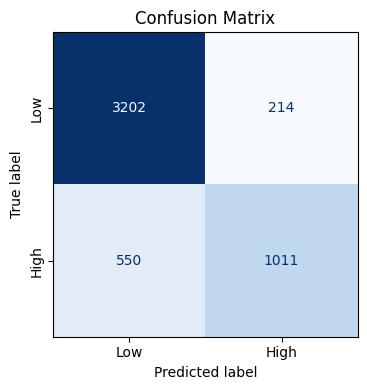
\includegraphics[width=0.30\textwidth]{plots/knn_binary_confmatrix.png}
    \caption{K-NN binary classification}
    \label{fig:binary_knn_confusion_matrix}
\end{wrapfigure}
The features used for the K-NN algorithm were normalized, as the model is sensitive to unscaled values: log-transformation (when needed) and \texttt{StandardScaler} were applied to data. 
Then, to perform this task, care was taken in selecting the appropriate type and amount of features to avoid unnecessary increased dimensionality.
For example, to provide the model with information about the origin of the titles, without introducing all 7 \texttt{countryOfOrigin\_[continent code]} attributes, only \texttt{countryOfOrigin\_freq\_enc} was kept. 
The remaining variables of the dataset were maintained as they offered diverse and non-redundant insights.\\
For this algorithm, a portion of the training set was held out as a validation set to enable external validation after internal cross-validation. 
A randomized hyperparameter search was indeed performed on the reduced training set, with each configuration evaluated using stratified 5-fold cross-validation. 
This process aimed to identify the optimal value of \textit{k} and explore additional algorithm parameters. 
The best configuration found is: \texttt{weights:'uniform', n\_neighbors:9, metric:'cityblock'}, which achieved the highest accuracy on the selected feature set.\\

The resulting model shows solid performance, achieving a test accuracy of 0.85. As expected, it performs better on the \textit{Low Engagement} class, with a high recall (0.94) and F1-score (0.89). 
In contrast, the \textit{High Engagement} class is more challenging for the model; while precision is reasonable (0.83), recall (0.65) indicates that a significant number of instances are misclassified as 
\textit{Low Engagement}.
This analysis is reflected in the confusion matrix in Figure~\ref{fig:binary_knn_confusion_matrix}, where 550 out of 1561 \textit{High Engagement} samples were incorrectly labeled as \textit{Low Engagement}.\\

To summarize, the macro average F1-score of 0.81 is suggesting that the model maintains a balanced performance across both classes.



\subsection{Naïve Bayes - Binary Classification}

\begin{wrapfigure}{l}{0.40\textwidth}
    \centering
    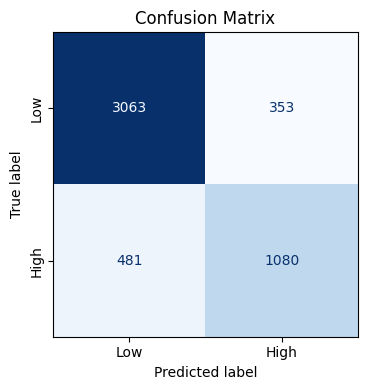
\includegraphics[width=0.30\textwidth]{plots/nb_binary_confmatrix.png}
    \caption{NB binary classification}
    \label{fig:nb_binary}
\end{wrapfigure}
For Naïve Bayes, a validation set was used to select the best feature set. Two variants were evaluated: GaussianNB and CategoricalNB. 
However, skewed distribution of continuous attributes and the relevance of discrete features (e.g., genres), made GaussianNB less suitable 
for the task, resulting in a slightly lower performance, in terms of accuracy and classification of underrepresented classes. 
Therefore, only CategoricalNB results are reported. 
To apply CategoricalNB, continuous features were discretized using meaningful bins, and each \texttt{countryOfOrigin\_[continent code]} feature was binarized (0 / $>$0), to maintain the only significant information; 
only \texttt{is\_from\_America\_bin} and \texttt{is\_from\_Europe\_bin} were used. Final features were encoded with OrdinalEncoder as required.
The results show good classification performance with an overall accuracy of 0.83, a solid outcome given the simplicity of the NB model.
However, differences between classes emerged: the \textit{Low Engagement} class performed better, with precision 0.87, recall 0.89, and F1 score 0.88, 
while the model struggled more identifying  \textit{High Engagement} examples, as confirmed by the low recall (0.70) for that value and by the 481 false 
negatives in the confusion matrix. The macro F1 average of 0.80, actually indicates a good balance overall, but some difficulty remains in handling the minority class.

% \begin{figure}[H]
%     \centering
%     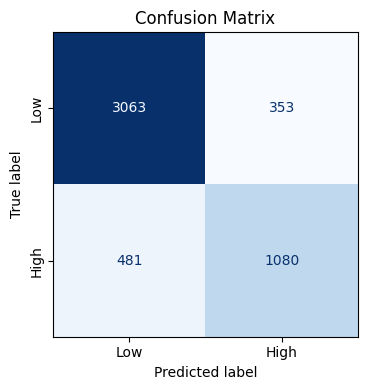
\includegraphics[width=0.30\linewidth]{plots/nb_binary_confmatrix.png}
%     \captionsetup{justification=centering, width=0.9\linewidth}
%     \caption{Naïve Bayes binary classification}
%     \label{fig:nb_binary}
% \end{figure}


\subsection{Decision Trees - Binary Classification}
For explainability purposes, features were not normalized nor transformed for the Decision Tree model,
as it does not require such preprocessing because it's not based on distance measures, but rather on
decision thresholds.\\
To identify the optimal hyperparameters, a Randomized Search was performed
using Repeated Stratified 5-Fold Cross-Validation with 10 repeats on the training set, optimized for
the macro-averaged F1-score.
The best configuration found used Gini index as the splitting criterion,
a maximum tree depth of 26, and a minimum of 3 samples per leaf.
The obtained decision tree is shown in figure~\ref{fig:binary_dt}.
\begin{figure}[H]
    \centering
    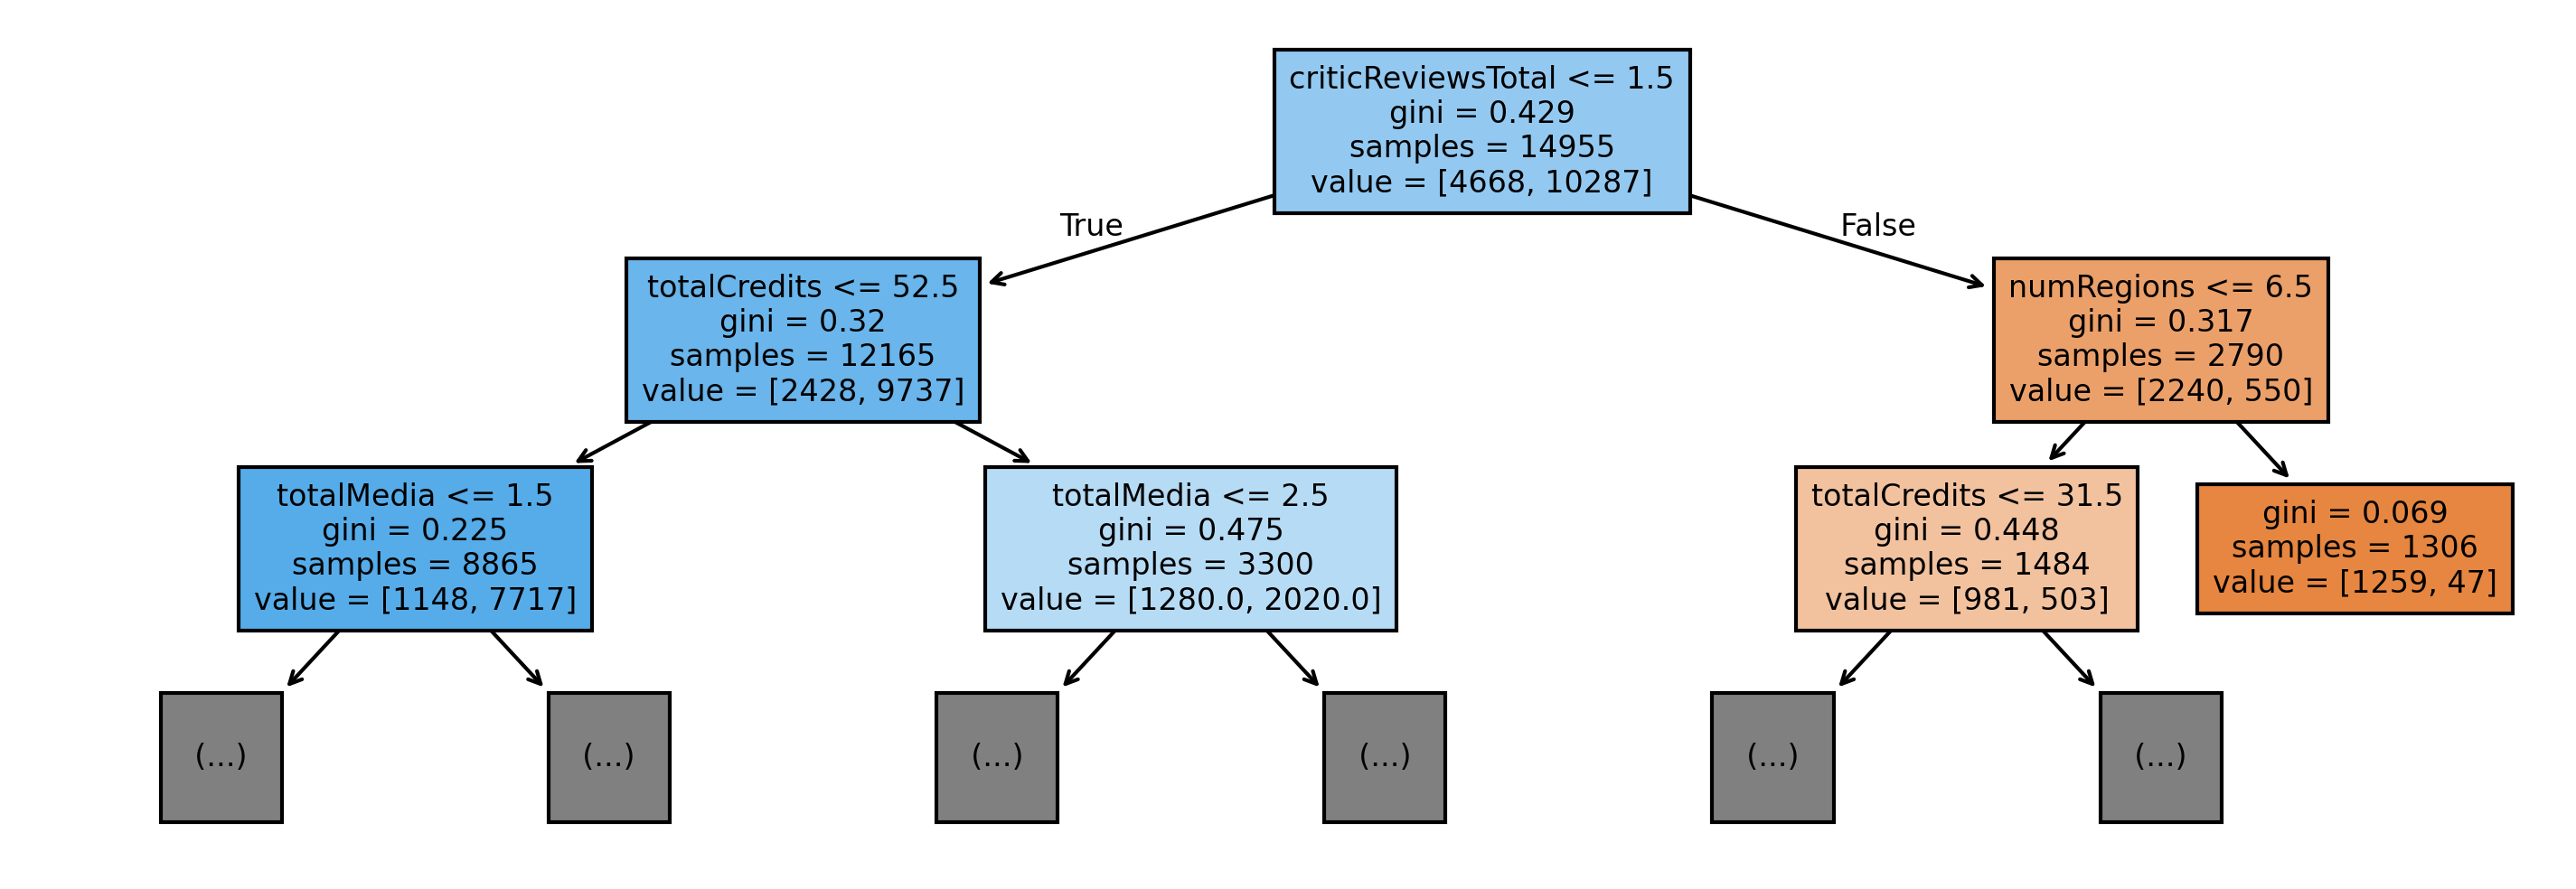
\includegraphics[width=0.8\linewidth]{plots/binary_dt.png}
    \captionsetup{justification=centering, width=0.9\linewidth}
    \caption{Decision Tree for binary classification}
    \label{fig:binary_dt}
\end{figure}

Unsurprisingly, the most important feature for the model was \texttt{criticReviewsTotal},
which amounted to 0.6 in the feature importance ranking. The following other 3 more important
features were \texttt{totalCredits} (0.15), \texttt{totalMedia} (0.10) and \texttt{numRegions} (0.09).
These four features take up around 93\% of the total feature importance, and are all present in the first
two splits shown in the Decision Tree.\\
% Classification performance is summarized in Table~\ref{tab:binary_classification_report}.

% \begin{table}[H]
%     \centering
%     \begin{tabular}{lcccc}
%         \toprule
%         \bf{Class} & \bf{Precision} & \bf{Recall} & \bf{F1-score} & \bf{Support} \\
%         \midrule
%         \bf{Low engagement} & 0.86 & 0.90 & 0.88 & 3416 \\
%         \bf{High engagement} & 0.75 & 0.69 & 0.72 & 1561 \\
%         \midrule
%         \bf{Macro avg} & 0.81 & 0.79 & 0.80 & \\
%         \bf{Weighted avg} & 0.83 & 0.83 & 0.83 & \\
%         \midrule
%         % & & \textbf{Train} & \textbf{Test} & \\
%         % \midrule
%         \bf{ROC AUC} & & & 0.87 & \\
%         \bf{Accuracy}  &  & & 0.83 & \\
%         \bottomrule
%     \end{tabular}
%     \caption{Classification report for binary classification}
%     \label{tab:binary_classification_report}
% \end{table}
Train performance was overall similar to the test performance; in particular, the respective accuracies
were of 0.83 and 0.84, and macro-F1 scores were 0.82 and 0.80.
In any case, post-pruning was tested, but did not yield any performance improvement, and was therefore
not applied.
The \textit{High Engagement} class showed low Recall values (0.71 on train set, 0.68 on test set).
This might be a consequence of class imbalance, as well as poor separability of the two classes.
This assumption is further supported by the
Precision scores of the class (0.78 on train, 0.75 on test).

% \begin{figure}[H]
%     \begin{minipage}{0.58\textwidth}
        % Figure~\ref{fig:conf_matr_binary_dt} shows the confusion matrix for the obtained
        % Decision Tree, with results regarding the test set.
        % As can be seen, a significant number of \textit{High Engagement} records was misclassified,
        % leading to a low Recall for that class.
        % This might be a consequence of class imbalance, as well as the possible presence
        % of noise in the data. It's also possible that the two classes are not well separated, leading
        % the model to prioritize the predominant class.\\
%     \end{minipage}
%     \hfill
%     \begin{minipage}{0.38\textwidth}
%         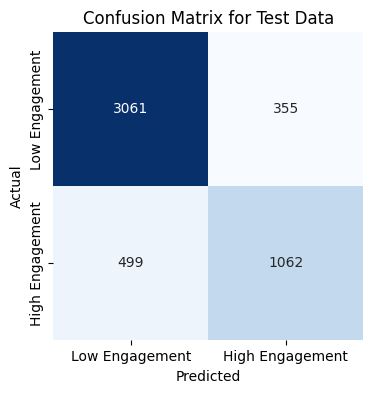
\includegraphics[width=\linewidth]{plots/binary_dt_confusion_matrix.png}
%         \captionsetup{justification=centering, width=0.9\linewidth}
%         \caption{Confusion matrix for binary classification}
%         \label{fig:conf_matr_binary_dt}
%     \end{minipage}
% \end{figure}

\subsection{Model Comparison - Binary Classification}
After applying the three algorithms to the binary classification task, it emerged that all models struggle to identify the minority class, 
\textit{High Engagement}, leading to lower recall values: 0.65 for K-NN, 0.70 for Naïve Bayes, and 0.69 for Decision Trees. 
This is confirmed by the confusion matrices, where many \textit{High Engagement} records are misclassified as \textit{Low Engagement}.\\

Among the models, K-NN handled the minority class best in terms of precision (0.83) and F1-score (0.73). 
However, the fact that Naïve Bayes performed the highest in terms of recall (0.70) makes it a more valid alternative in scenarios where preventing 
high-engagement titles from being misclassified as low-engagement ones is a priority. In general, Decision Trees show similar performances to Naïve Bayes for all metrics
In conclusion, K-NN is still considered the most efficient model for this task, as it also achieves the highest overall accuracy, 
the best macro-average F1-score and the most balanced results across both classes. 
The macro-average ROC AUC scores for all three models are also quite similar, with K-NN showing the highest value (0.89), 
followed by Naïve Bayes (0.88) and Decision Trees (0.87).
A summary of the results of the best model is presented in Table~\ref{tab:best_model_binary_classification}.

% After having performed the task using the three algorithms, some interesting aspects emerged.
% As expected, all the models, to a different extent, struggle to identify the minority class, \textit{High Engagement}, resuling in lower recall values
% - 0.65 for K-NN, 0.70 for Naïve Bayes, and 0.68 for Decision Trees.
% This is evident in the confusion matrices, where a significant number of \textit{High Engagement} records are misclassified as \textit{Low Engagement}.
% In particular, K-NN handled the minority class the best in terms of precision and F1-score, achieving respectively 0.83 and 0.73.
% However, the fact that Naïve Bayes performed better in terms of recall (0.70) makes it a more valid alternative
% in scenarios where preventing high-engagement titles from being misclassified as low-engagement ones is a priority.
% Decision Trees are located in the middle, showing similar performances to Naïve Bayes, but having a slightly lower recall.
% In conclusion, considering all these aspects, K-NN is still considered the most efficient model for this task, as it also performs best globally. 
% In the table~\ref{tab:best_model_binary_classification} its overall results are summarized.
\begin{table}[H]
    \centering
    \begin{tabular}{cccccc}
        \toprule
        \bf{} & \bf{Accuracy} & \bf{Precision Macro Avg} & \bf{Recall Macro Avg} & \bf{F1-score Macro Avg} & \bf{AUC} \\
        \midrule
        \textbf{K-NN} & 0.85 & 0.84 & 0.79 & 0.81 & 0.89\\
        \bottomrule
    \end{tabular}
    \caption{Overall metrics - K-NN}
    \label{tab:best_model_binary_classification}
\end{table}





% \begin{table}[H]
%     \centering
%     \begin{tabular}{lcccccc}
%         \toprule
%         \bf{Model} & \bf{Precision} & \bf{Recall} & \bf{F1-score} & \bf{Accuracy} \\
%         \midrule
%         K-NN (Low Eng) & 0.83 & 0.65 & 0.72 & 0.85 \\
%         K-NN (High Eng) & 0.87 & 0.94 & 0.89 & 0.85 \\
%         \midrule
%         Naïve Bayes (Low Eng) & 0.74 & 0.70 & 0.72 & 0.83 \\
%         Naïve Bayes (High Eng) & 0.87 & 0.89 & 0.88 & 0.83 \\
%         \midrule    
%         Decision Tree (Low Eng) & 0.86 & 0.90 & 0.88 & 0.84 \\
%         Decision Tree (High Eng) & 0.75 & 0.68 & 0.72 & 0.84 \\
%         \bottomrule
%     \end{tabular}
%     \caption{Binary classification - performance comparison}
%     \label{tab:binary_classification_comparison}
% \end{table}





%%%%%%%%%%%%%%%%%%%%%%%%%%%%%%%%%%%%%%%%%%%%%%%%%%%%%%%%%%%%%%%%%%%%%%%%%%%%%%%%%%%%%%%%%%%%%%%%%%%%%%%%%%%%%5555
\section{Multiclass classification}\label{sec:multiclass_classification}
Among the multiclass features in the training set, \texttt{titleType} was selected as the target variable
for this task, due to its relevance within the dataset. Because of their strong correlation with
\texttt{titleType}, the feature \texttt{canHaveEpisodes} and the genre \textit{Short} were excluded from the
feature set. Furthermore, since the primary imputation method for missing values in \texttt{runtimeMinutes}
relied on information from the chosen target variable, these values were re-imputed to avoid data leakage.
Specifically, missing entries were filled by sampling from the overall distribution of
\texttt{runtimeMinutes}, without referencing \texttt{titleType} itself.\\

One final point to note is the imbalance in the target feature (previously shown in
figure~\ref{fig:titleType_distrib}), which was explicitly taken into account
during the design of the models. As for the binary classification task, macro-averaged F1-score was
a key metric for model evaluation, as it provides a balance between each class's precision and recall.




% This feature was created to impute the missing values of the original \texttt{runtimeMinutes} variable,
% but without using the median value according to the titleType. Instead, the missing values were imputed using the help of two variables: \texttt{canHaveEpisodes} and \texttt{is\_Short}
% (as one of the resulting variables of the multi-label one-hot encoding process of the \texttt{genres} attribute).
% In particular, 
% \textbf{SCRIVERE COME E' STATA IMPUTATA NO\_TT - con canhaveepisodes e is\_short preso dai generi}.
% This approach prevents a significant error, as it would be methodologically incorrect to use \texttt{titleType}-based 
% imputation for an attribute when \texttt{titleType} itself is the target variable to predict.
\subsection{K-NN - Multiclass Classification}
% For the multiclass classification task using the K-NN algorithm, the inclusion of a broad set of 
% features is necessary and justified, as it was found to help the model to better distinguish between 
% underrepresented classes - even if the results in their classification are not optimal. 
% Even though the choice of keeping those classes lowers the overall performance (accuracy) of the model, 
% it is a trade-off in favor of larger coverage and sensitivity across all classes.\\
% The hyperparameter tuning strategy that was employed is the same as in binary classification with K-NN. 
% The configuration that achieved the best performances is: \texttt{{weights:'uniform', n\_neighbors:12, metric:'cityblock'}}.\\ 
% As expected, the model shows mixed performances across the different classes. 
% The overall test accuracy reaches 0.76, which is a respectable result for a multiclass problem. 
% However, since accuracy is a global metric, more attention should be paid to the performances of the single classes. 
% Classes with a larger support, like \textit{tvEpisode} (1596) and \textit{movie} (1848), are handled quite well: \textit{tvEpisode} reaches an F1-score of 0.83 and \textit{movie} 0.84, both supported by high recall values (respectively 0.93 and 0.87). 
% \begin{figure}[H]
%     \centering
%     \begin{minipage}[t]{0.59\textwidth}
%         \vspace{0pt}
%         This is also clearly visible in the confusion matrix of Figure~\ref{fig:multiclass_knn_confusion_matrix}, where these classes dominate with a high count of correct predictions. 
%         On the other hand, the model struggles with 2 classes in particular: \textit{tvMiniSeries} and \textit{tvSpecial}, i.e. the classes with the least support (respectively 68 and 42). 
%         In particular, \textit{tvMiniSeries} shows a very low recall (0.03), meaning that it is rarely correctly identified. 
%         Similarly, \textit{tvMovie} is mostly misclassified, showing a low F1-score of 0.29.\\
        
%         An interesting trend to notice in the confusion matrix is how records belonging to class \textit{tvSeries} are frequently misclassified as \textit{tvEpisodes}. 
%         This is likely due to the similar nature between the two, as both refer to television content and often share overlapping characteristics, considering also that a tv episode is basically part of a tv series. 
%         A similar confusion occurs between \textit{tvMovie} and \textit{movie}.\\

%         To summarize, since the model achieves a macro average F1-score of 0.50, this reflects clearly this imbalance in performance: while the model performs well on the majority classes, it fails to generalize well especially the minority ones.
%     \end{minipage}
%     \hfill
%     \begin{minipage}[t]{0.40\textwidth}
%         \vspace{0pt}
%         \centering
%         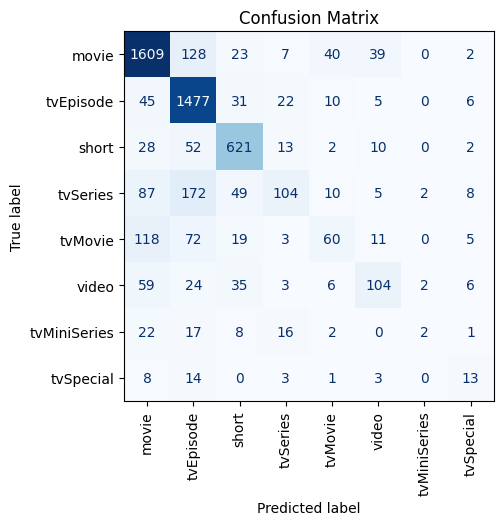
\includegraphics[width=\linewidth]{plots/knn_multiclass_confmatrix.png}
%         \captionsetup{justification=centering, width=0.65\linewidth}
%         \caption{K-NN multiclass classification}
%         \label{fig:multiclass_knn_confusion_matrix}
%     \end{minipage}
% \end{figure}
% \vspace{-0.8em}



\begin{wrapfigure}{l}{0.4\textwidth}
    \centering
    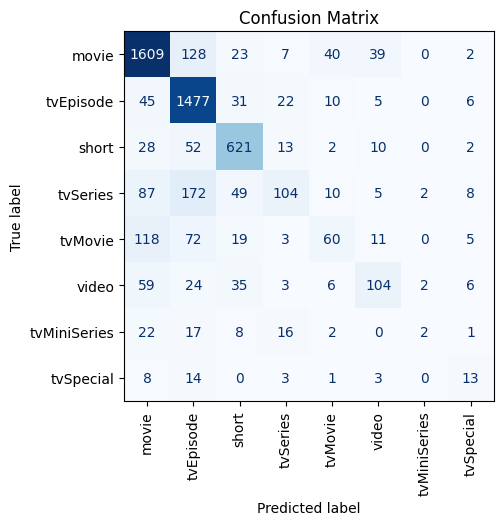
\includegraphics[width=0.35\textwidth]{plots/knn_multiclass_confmatrix.png}
    \caption{K-NN confusion matrix}
    \label{fig:multiclass_knn_confusion_matrix}
\end{wrapfigure}
For the multiclass classification task using the K-NN algorithm, the inclusion of a broad set of 
features is necessary and justified, as it was found to help the model to better distinguish between 
underrepresented classes - even if the results in their classification are not optimal. 
Even though the choice of keeping those classes lowers the overall performance (accuracy) of the model, 
it is a trade-off in favor of larger coverage and sensitivity across all classes.
The hyperparameter tuning strategy that was employed is the same as in binary classification with K-NN. 
The configuration that achieved the best performances is: \texttt{{weights:'uniform', n\_neighbors:12, metric:'cityblock'}}.\\ 

As expected, the model shows mixed performances across the different classes. 
The overall test accuracy reaches 0.76, which is a respectable result for a multiclass problem. 
However, since accuracy is a global metric, more attention should be paid to the performances of the single classes. 
Classes with a larger support, like \textit{tvEpisode} (4690 records in the training set) and \textit{movie} (5442), are handled quite well: \textit{tvEpisode} reaches an F1-score of 0.83 and \textit{movie} 0.84, both supported by high recall values (respectively 0.93 and 0.87). 
This is also clearly visible in the confusion matrix of Figure~\ref{fig:multiclass_knn_confusion_matrix}, where these classes dominate with a high count of correct predictions. 
On the other hand, the model struggles with 2 classes in particular: \textit{tvMiniSeries} and \textit{tvSpecial}, i.e. the classes with the least support (respectively 186 and 158). 
In particular, \textit{tvMiniSeries} shows a very low recall (0.03), meaning that it is rarely correctly identified. 
Similarly, \textit{tvMovie} is mostly misclassified, showing a low F1-score of 0.29.\\
% forse rimetti i dati -> non messi sotto
% An interesting trend to notice in the confusion matrix is how records belonging to class \textit{tvSeries} are frequently misclassified as \textit{tvEpisodes}. This is reflected in a very low recall (0.24) for \textit{tvSeries} and in a quite high precision (0.76) for \textit{tvEpisode}.
% This is likely due to the similar nature of the two, as both refer to television content and often share overlapping characteristics, considering also that a tv episode is can be considered part of a tv series. 
% A similar confusion occurs between \textit{tvMovie} and \textit{movie}.\\
To summarize, since the model achieves a macro average F1-score of 0.50, this reflects clearly this imbalance in performance: while the model performs well on the majority classes, it fails to generalize well especially the minority ones.




\subsection{Naïve Bayes - Multiclass Classification} 
For the multiclass classification task, the same procedure as binary classification (explained in Subsection 3.1.2) were applied. 
Note that including genre features, significantly improved classification across all classes, particularly those with limited support in the training set. 
Under GaussianNB, tvMiniSeries (68 objects) was not classified at all, and tvMovie (288) and tvSpecial (42) were poorly classified. 
With CategoricalNB, which better handles categorical data, these classes showed improvements, confirming its suitability for this task.\\   
\begin{wrapfigure}{r}{0.4\textwidth}
    \centering
    \captionsetup{justification=raggedleft, width=1\linewidth}
    \caption{NB confusion matrix}
    \label{fig:nb_multiclass}
    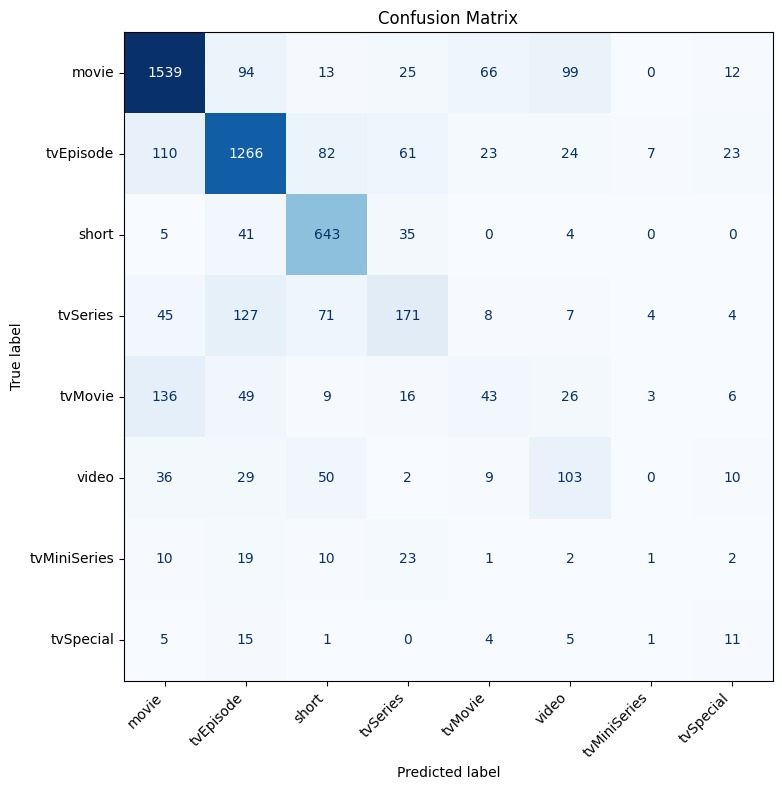
\includegraphics[width=0.9\linewidth]{plots/nb_multiclass_confmatrix.jpg}
\end{wrapfigure}
The model achieves an overall accuracy of 0.73, reasonable for multiclass classification, but indicative of difficulties in handling all categories equally. 
High F1-scores (about 0.80) for frequent classes like \texttt{movie}, \texttt{tvEpisode}, and \texttt{short} suggest effective recognition, likely due to their prevalence and distinctive traits. 
The \texttt{movie} class also shows strong precision (0.82) and recall (0.84), confirming the model’s reliability on this category.
As expected, performance drops for underrepresented classes: \texttt{tvMiniSeries}, \texttt{tvSpecial}, and \texttt{tvMovie}  have low F1-scores (respectivly 0.02, 0.21, 0.17). 
Other than their low support, this is probably linked to the presence of common features with more dominant classes, such as \texttt{tvEpisode} or \texttt{Movie} (e.g., 140 \texttt{tvMovie} instances misclassified as movie). 
The \texttt{tvSeries} class also shows issues, with moderate precision (0.52) but low recall (0.40), indicating many missed instances.
The very low macro F1-score actually reflects the inability of the model to perform in a balanced way on all the classes, 
while the higher weighted F1-score (0.71) , suggests that the majority classes have a greater influence on overall performance than the minorities.

% \begin{figure}[H]
%     \centering
%     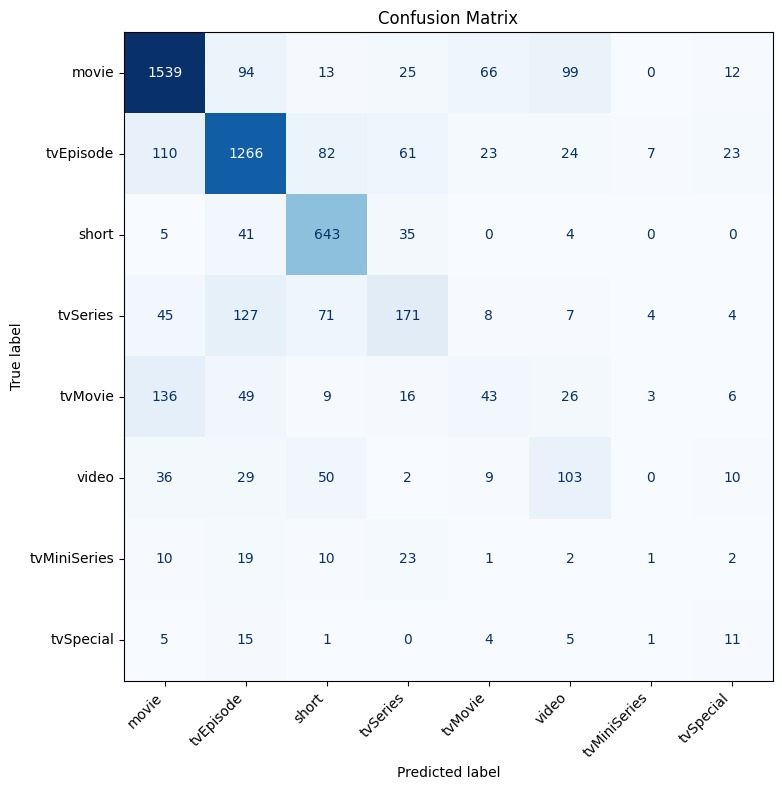
\includegraphics[width=0.30\linewidth]{plots/nb_multiclass_confmatrix.jpg}
%     \captionsetup{justification=centering, width=0.9\linewidth}
%     \caption{Naïve Bayes multiclass classification}
%     \label{fig:nb_multiclass}
% \end{figure}



\subsection{Decision Trees - Multiclass Classification}
Like for the binary classification task, the Decision Tree model was trained without normalizing or
transforming the features, making the model more interpretable. Feature selection was performed by studying
feature importance, while hyperparameters were optimized with a Randomized Search,
which used Repeated Stratified 5-Fold Cross-Validation with 5 repeats on the training set, optimized for
the macro-averaged F1-score.
The best configuration found used Entropy as splitting criterion, had a max depth of 14, a minimum of
5 samples per leaf, and a minimum of 8 samples in order to split an internal node.
\begin{figure}[H]
    \centering
    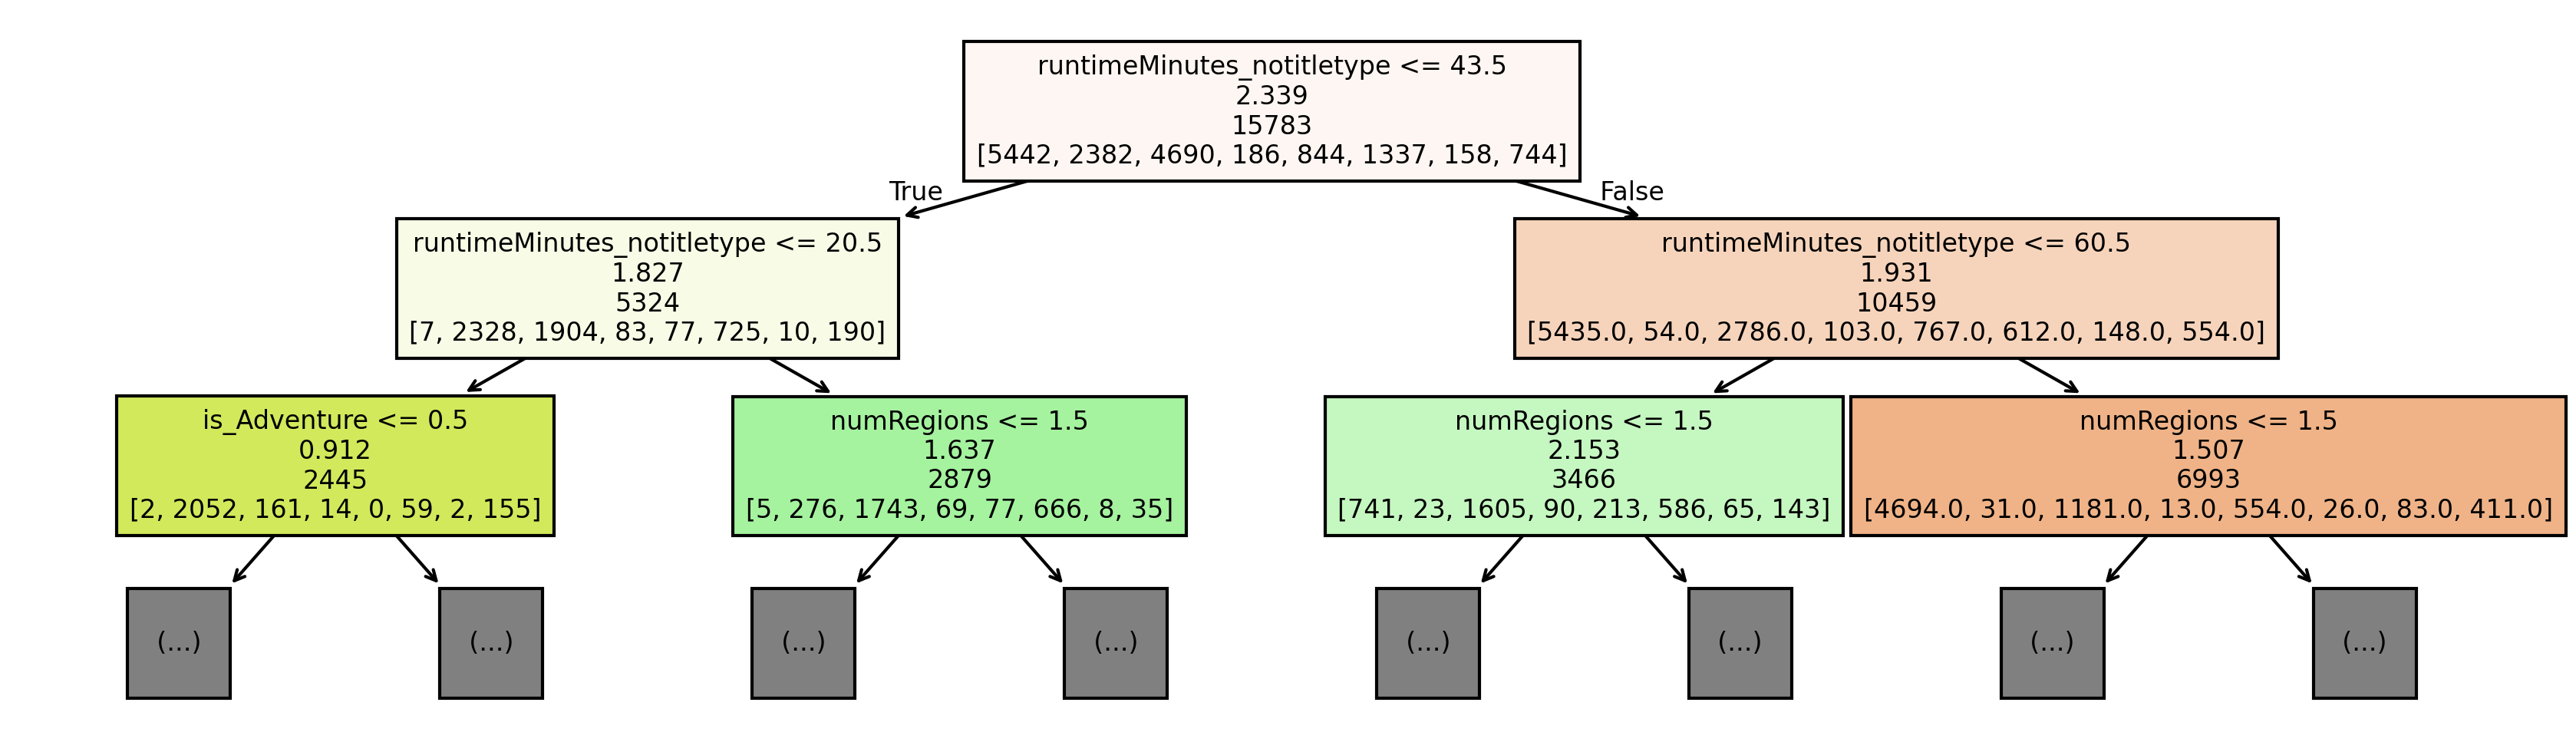
\includegraphics[width=0.88\linewidth]{plots/multiclass_tree.png}
    \captionsetup{justification=centering, width=0.9\linewidth}
    \caption{Decision Tree for multiclass classification}
    \label{fig:multiclass_dt}
\end{figure}
Figure~\ref{fig:multiclass_dt} shows the Decision Tree obtained for the multiclass classification task.
The most important feature for the model was \texttt{runtimeMinutes}, on which the first two levels
of the tree are based, with a feature importance of 0.45.
Three out of the four splits in the following level are based on \texttt{numRegions} being smaller than
2, giving the feature an importance of 0.13; the fourth is based on the \textit{Adventure} genre,
which has an importance of 0.01.
\begin{wrapfigure}{r}{0.4\textwidth}
    \centering
    \captionsetup{justification=raggedleft, width=1\linewidth}
    \caption{DT Confusion matrix}
    \label{fig:multiclass_dt_conf_matrix}
    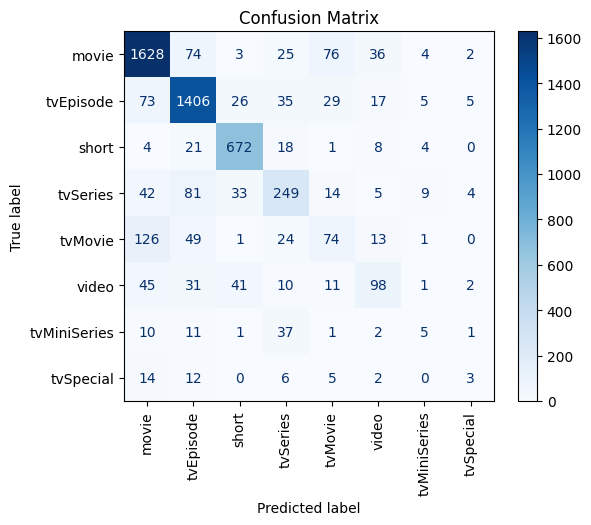
\includegraphics[width=0.9\linewidth]{plots/multiclass_dt_conf_matrix.png}
\end{wrapfigure}
The model showed a general tendency towards overfitting, and many configurations were tested to prevent
this.
The overall accuracy shows a significant drop (from 0.86 on the train set, to 0.75 on the test set),
as well the macro-averaged F1-score, going from 0.65 to 0.52.
This was given from the \textit{tvMiniSeries} and \textit{tvSpecial} classes: these had f1-scores of
0.35, 0.22 respectively on the train set, and both had 0.10 on the test set. Since they were by far
the least represented classes, they required a trade-off between low-represented classes classification
and generalization. This can be seen in figure~\ref{fig:multiclass_dt_conf_matrix}, which shows the fact
that most predictions for these classes were misclassified.\\
In order to mitigate overfitting, post-pruning was tested, but did not give particular benefits.
Higher values for the parameter $\alpha$ had minor positive effects on the generalization
capabilities of the models, at the cost of losing predictions on the less represented classes.
Another aspect highlighted by the confusion matrix is the fact that \textit{tvMovie} was often
classified as \textit{movie}, leading to a Recall value of 0.26 on the test set.
This is likely due to the fact that the two classes are overlapping, since they are semantically related,
and is further supported by the fact that the most common misclassification for \textit{movie} was
\textit{tvMovie}, albeit with a low number of occurrences, likely due to it being the biggest class.
A similar case can be made for \textit{tvSeries} and \textit{tvMiniSeries}, with 37 out of the total 68
of the \textit{tvMiniSeries} records being misclassified as \textit{tvSeries}.


\subsection{Model Comparison - Multiclass Classification}
% As expected, a common issue that was observed is the difficulty in correctly classifying underrepresented classes.
% Classes such as \textit{tvMiniSeries} (186 records in the training set), \textit{tvMovie} (844), and \textit{tvSpecial} (158) consistently show low recall and F1-scores across all models.
% The poorest performance is observed for the first one, with recall values ranging from 0.01 (Naïve Bayes) to 0.07 (Decision Trees), and a maximum F1-score of 0.10 (Decision Trees).
% On the other hand, well represented classes, such as \textit{movie} (5442 records in the training set) and \textit{tvEpisode} (4690), are generally classified accurately, as previously discussed.\\
The analysis of Decision Tree, Categorical Naïve Bayes, and K-NN models reveals several consistent patterns in their performances. 
As expected, underrepresented classes like  \textit{tvMiniSeries} (186 records in the training set), \textit{tvMovie} (844), and \textit{tvSpecial} (158) show consistently low recall and F1-scores across all models.
 \textit{tvMiniSeries} performs worst, with recall between 0.01 (Naïve Bayes) and 0.07 (Decision Trees), and a maximum F1-score of 0.10. 
 In contrast, well-represented classes like  \textit{movie} (5442) and\textit{tvEpisode}(4690) are always classified accurately. However, class imbalance alone does not fully explain the misclassifications. The confusion matrices showed systematic misclassification patterns, 
where minority classes were frequently absorbed into semantically related but more dominant categories. 
Across all models, but at different extent, \textit{tvMovie} is frequently confused with \textit{movie}, and \textit{tvMiniSeries} is often predicted as \textit{tvSeries}, e.g. resulting in 37 out of 68 instances misclassified by Decision Trees.
K-NN also shows a tendency to predict \textit{tvSeries} as \textit{tvEpisode}.\\
Decision Tree achieved the best overall performance (0.79 accuracy, 0.52 macro average F1), followed by K-NN and Naïve Bayes. 
However, the ROC analysis reveals an apparent paradox: Naïve Bayes showed the highest macro-average AUC (0.91), despite poorer classification results.
Despite this, Decision Tree remains the optimal choice, effectively balancing overall accuracy with minority class performance, 
since relying only on AUC can be misleading in imbalanced multiclass scenarios.
In Table~\ref{tab:best_model_multiclass_classification} its overall results are summarized.
\begin{table}[H]
    \centering
    \begin{tabular}{cccccc}
        \toprule
        \bf{ } & \bf{Accuracy} & \bf{Precision Macro Avg} & \bf{Recall Macro Avg} & \bf{F1-score Macro Avg} & \bf{AUC} \\
        \midrule
        \bf{DT} & 0.79 & 0.55 & 0.51 & 0.52 & 0.84 \\
        \bottomrule
    \end{tabular}
    \caption{Overall metrics - Decision Tree}
    \label{tab:best_model_multiclass_classification}
\end{table}


 






% Because of class imbalance, for evaluation purposes, macro-averaged F1-score was heavily considered.